% [4~r\textsuperscript{o}]
\pstart%
\begin{wrapfigure}[11]{l}{0.38\textwidth}                    
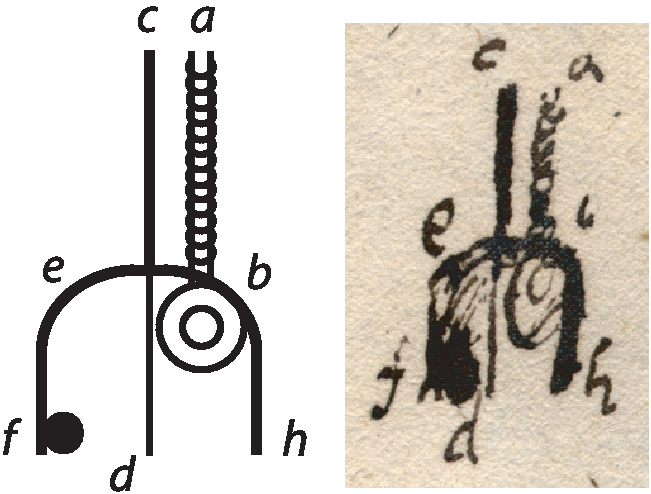
\includegraphics[trim = 0mm 0mm -5mm 0mm, clip,width=0.38\textwidth]{images/lh0040104b_004r1.pdf}\\
\centering [\textit{Fig. 4}]
\end{wrapfigure}%
Notavi in tertio vitulo recens nato, et in cujus ventriculo nondum lac cernebatur, sed materies quaedam ex viridi nigrescens, ejus intestinum rectum supra modum fuisse inflatum et solo flatu impletum supra vero aliud intestinum fuisse quadam materia nigra plenum et multo angustius. Vesica etiam erat ingens, et multum aquae continebat. Hepar vero minus erat quam praecedentis et ejus caro super umbilicum minus extuberabat; et fel minus ab eo removebatur, lien vero dorsum (+ an deorsum? +) versus in sinistra parte vergebat.
\pend%
\newpage
\pstart%
Aspera arteria non erat tam dura quam praecedens, cristamque etiam habebat ut praecedens. % \edtext{}{\lemma{praecedens}\Cfootnote{Vgl. LH IV 1,4B Bl. 3v\textsuperscript{o}, Z. 12, hier S. ??.}}
Cui a sinistris gula incumbebat; gulae autem truncus aortae descendentis amplissimus, eratque ad huc magis a sinistris quam gula.
\pend
\pstart
$ab$ aspera arteria, $bef$ truncus cavae descendentis; $cd$ gula, $gh$ vena cava ab hepate $h$ ad cordis partem $g$ ascendens.
\newline%
\indent%
Pulmo dexter in duobus asperae arteriae locis ejus vasa admittebat, sinister vero tantum in uno loco, qui respondebat parti inferiori dextri lateris infra truncum aortae descendentis, adeo ut videretur initio aortam ex anteriore thoracis parte versus sinistram partem ac deinde in dorsum supra pulmonem sinistrum ascendisse priusquam ex dorso viam sibi rursus fecisset, adeoque sinistrum pulmonem amplectendo ejus vasa ex aspera arteria venientia depressisse; apparebant autem, excisis scilicet pulmonibus inter ora, vasorum in illos ingredientium duo insignia utrinque
\edtext{unum}{\lemma{}\Afootnote{\textit{Am Rand}: \Denarius}}
e regione posita quae videbantur esse venae arteriosae partes eratque sinistrum immediate infra truncum aortae descendentis, infra haec utrinque etiam unum insigne erat, quod videbatur esse ex arteria venosa, sed in sinistro latere videbantur esse plures alii, nec praecipuum erat tam insigne quam in dextro quae unde revera prodierint, ablato pericardio cognoscam.
\pend%
\pstart%
Antequam pericardium tollerem manifeste observavi nervum qui a collo supra dextram partem pericardii anterius ad dia$\phi$ragma descendebat, sed et alium quoque supra sinistram partem pericardii eodem fere modo ad dia$\phi$ragma ibat nisi quod priusquam ejus carnem ingrederetur in duas partes scindebatur, in ipsam enim dia$\phi$ragmatis carnem utrinque penetrabant, et ibi absumebantur. Circa lienem observavi ejus partem quae erat versus spinam esse incurvam et intus velut exulceratam (ut etiam erat in praecedenti) et in postrema ejus parte paulo crassiorem, in medio ejus curvitatis erant simul ingressus omnium vasorum, id est venae insignis, arteriae item insignis, et nervi, unde videtur aperte ostendi lien in medio posterioris partis initio fuisse genitum et postea ibi fuisse protrusum, jecore in dextram partem recedente. Pericardium tribus membranis tenuissimis alligabatur, quarum una sursum videbatur esse intersepiens, vel alia infra intersepientem adnata, nec notavi essetne simplex vel duplex: duae autem aliae inferiores a dia$\phi$ragmate una simul cum vena cava, alia sinistra cum oesophago et aorta (quae ibi oblonga quadam glandula interjecta separabantur, et aorta magis versus spinam dorsi erat) ascendebant: Erant autem hae duae membranae in pericardio parvi digiti latitudine ab invicem sejunctae, unaquaeque duplex, et ex his omnibus simul membranis alia circa totum pericardium producta erat, multis quasi glandulis vel adipe conspersa, quam totam a pericardio separavi. Separavi deinde cavam a dia$\phi$ragmate, et notavi ramum exiguum ab illa in dia$\phi$ragma permeantem, moxque in duos et plures ramos dispersum. Separavi oesophagum ab eodem, notavique duo vasa insignia (quos puto nervos sexti paris) simul cum oesophago descendentia. Separavi deinde aortam quam vidi per aliud foramen transire quam oesophagum, nempe juxta spinam, nec ullum aliud vas cum illa animadverti. Separavi deinde nervos oesophagi quos omnes agnovi ab eadem origine esse; unus tamen superior in duos versus cerebrum dividebatur qui duo utrinque per pulmones et pericardium fibras mittebant, sed et recurrentes ad asperam arteriam et alter inferior vel ab istis duobus vel ab uno saltem pro certo veniebat.
\pend%
\pstart%
Separavi deinde oesophagum quem vidi distincte per latus sinistrum asperae arteriae descendentem accurate in medio inter utrumque pulmonem descendere, adeo ut ejus descensu pulmones viderentur esse divisi.
\pend%
\pstart%
\begin{wrapfigure}[12]{l}{0.38\textwidth}                    
\includegraphics[trim = 0mm -3mm -5mm 0mm, clip,width=0.38\textwidth]{images/lh0040104b_004r2.pdf}\\
\centering [\textit{Fig. 5}]
\end{wrapfigure}%
Discidi postea pericardium constans membrana tenui quidem sed tensa et quasi cornea, utrinque laevi et polita (: detracta nempe supra eam membrana ex pleura :) in eo humor adhuc aliquis erat. Nulli parti cordis versus mucronem adhaerebat, sed circumquaque basi et ejus vasis et asperae arteriae sive pulmonibus tam firmiter adhaerebat, ut fuerit abscindenda, frangebantur enim vasa cum illam volebam avellere; notavi autem primo illam trunco cavae versus hepar ita firme annecti huncque truncum qui totam aurem dextram amplectens trunco aortae ascendenti et ramo venae arteriosae adhuc intra pericardium existens
\edtext{jungebatur conscendere}{\lemma{}\Bfootnote{jungebatur\ \textbar\ :) \textit{gestr.}\ \textbar\ conscendere \textit{L}}}
et illa in parte ex pulmonibus egredi, adeo ut non adhaereret trunco cavae nisi in ejus ingressu et egressu adhaerebat eodem modo aortae et venae arteriosae
in [illarum]\edtext{}{\lemma{illorum}\Bfootnote{\textit{L \"{a}ndert Hrsg.}}}
egressu sed ita firmiter ut sursum adducta appareret illam ex corde egredi, deorsum vero e regione quidem vasorum ex ipsis vasis alibi ex pulmonibus. Separavi deinde asperam arteriam notavique illam cordi non adhaerere, nisi mediante pulmonum corpore, item in illa tres esse insigniter distinctas partes per quas pulmonibus jungebatur, duas scilicet $a$ et $b$ in dextro;
\edtext{[3\textsuperscript{tiam}]}{\lemma{3\textsuperscript{tia}}\Bfootnote{\textit{L \"{a}ndert Hrsg.}}}
in sinistro. Caro autem pulmonum adhaerens pericardio admittebat vasa e corde ex quatuor locis quorum duo $d$ et $e$ jungebantur vasis ex $c.$
$f$ vero jungebatur cum $b$ et $g$ cum $a,$
et truncus aortae descendentis erat in medio $h$ versus anteriorem partem descendebatque versus $i$ deprimendo $d$ et $e.$
%\begin{wrapfigure}{l}{0.15\textwidth}                    
%\includegraphics[width=0.15\textwidth]{images/lh004_01_4b_004r3.pdf}
%\caption{Bildbeschreibung}
%\end{wrapfigure}
Item vasa asperae arteriae egrediebantur quidem paulo magis ex posteriori parte ejus quam ex anteriori, sed postea paulo magis in anteriorem flectebantur quamquam hoc non ita videatur effatu dignum.
[4~v\textsuperscript{o}]
\pend
%\count\Bfootins=1500
%\count\Cfootins=1500
%\count\Afootins=1500